\subsection{Heurística}

\texttt{euclideanHeuristic} ya viene provista en \texttt{searchAgents.py} (tampoco fue necesario
implementarla):

\begin{figure}[H]
\centering
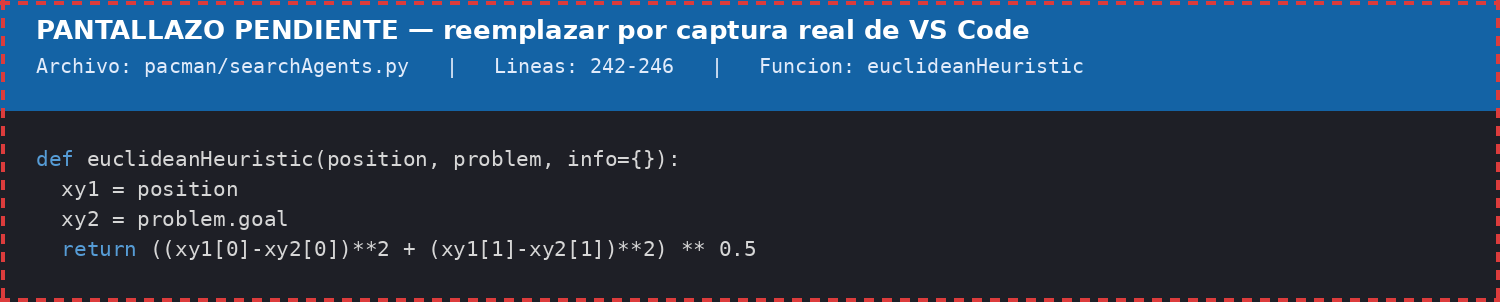
\includegraphics[width=0.8\textwidth]{capturas/actividad06_euclidiana.png}
\caption{\texttt{euclideanHeuristic} en \texttt{pacman/searchAgents.py} (líneas 242-246).}
\label{fig:act06-euclidiana}
\end{figure}

Calcula $h_E(n) = \sqrt{(x_n-x_g)^2 + (y_n-y_g)^2}$: la distancia en línea recta entre $n$ y la
meta, ignorando también las paredes (por lo tanto también es admisible, por el mismo argumento que
Manhattan: nunca sobreestima el costo real).

\subsection{Procedimiento y resultados}

Se ejecutó A* con las tres heurísticas (nula, Manhattan y Euclidiana) sobre \texttt{mediumClassic}
(ver \texttt{experimentos/actividad6\_euclidiana.py}).

\begin{table}[H]
\centering
\caption{Comparación de heurísticas con A*}
\label{tab:act6-comparacion}
\begin{tabular}{lrrrr}
\toprule
\textbf{Heurística} & \textbf{Longitud} & \textbf{Costo} & \textbf{Expandidos} & \textbf{Tiempo (s)} \\
\midrule
$h(n)=0$      & 12 & 12 & 69 & 0.000262 \\
Manhattan     & 12 & 12 & 15 & 0.000066 \\
Euclidiana    & 12 & 12 & 16 & 0.000070 \\
\bottomrule
\end{tabular}
\end{table}

Las tres heurísticas encuentran el mismo costo óptimo (12): las tres son admisibles, así que A*
sigue siendo óptimo con cualquiera de ellas. La diferencia está en cuánto ayudan a reducir la
exploración: Manhattan expande 54 nodos menos que $h(n)=0$ (69 $\rightarrow$ 15) y Euclidiana 53
menos (69 $\rightarrow$ 16). Manhattan es, además, ligeramente mejor que Euclidiana (15 vs. 16
nodos expandidos) en este layout.

\subsection{Pregunta de análisis}

\textbf{Pac-Man se desplaza únicamente horizontal o verticalmente. ¿Cuál de las dos heurísticas
representa mejor este tipo de movimiento? Justifique su respuesta utilizando los resultados
experimentales.}

Manhattan representa mejor el movimiento de Pac-Man, y los resultados experimentales lo confirman:
expandió 15 nodos frente a los 16 de Euclidiana para llegar al mismo costo óptimo. La razón es que
$h_E(n) \le h_M(n)$ para cualquier par de puntos (la distancia en línea recta nunca es mayor que la
suma de catetos ortogonales; es la desigualdad triangular aplicada a un triángulo rectángulo). Como
Pac-Man solo puede moverse en las 4 direcciones cardinales --nunca en diagonal--, el costo real de
moverse entre dos celdas siempre coincide con su distancia Manhattan (cuando no hay paredes de por
medio) y nunca con su distancia Euclidiana, que es una subestimación adicional e innecesaria en
este espacio de acciones. Dicho de otro modo: Euclidiana está diseñada para un agente que puede
moverse en línea recta en cualquier ángulo, algo que Pac-Man no puede hacer; al aplicarla aquí,
subestima el costo real más de lo que Manhattan lo hace, y una heurística que subestima más aporta
menos información para podar la búsqueda --- por eso expande más nodos.

Esta misma conclusión se repite en \texttt{openClassic} (Cuadro~\ref{tab:act3-verificacion}, donde
la diferencia es mucho más marcada: 27 nodos con Manhattan frente a 31 con Euclidiana), lo que
descarta que la ventaja de Manhattan en \texttt{mediumClassic} sea casualidad de ese layout en
particular.
